% !TEX root = ../thesis-example.tex
%
\chapter{Resultados}
\label{Resultados}




\section{Resultado del calculo de entropias}

Se usaron los dato DDJA....
Los preciosse pueden observar en laFigura \ref{precioseps}.....


\begin{figure}
	\centering
	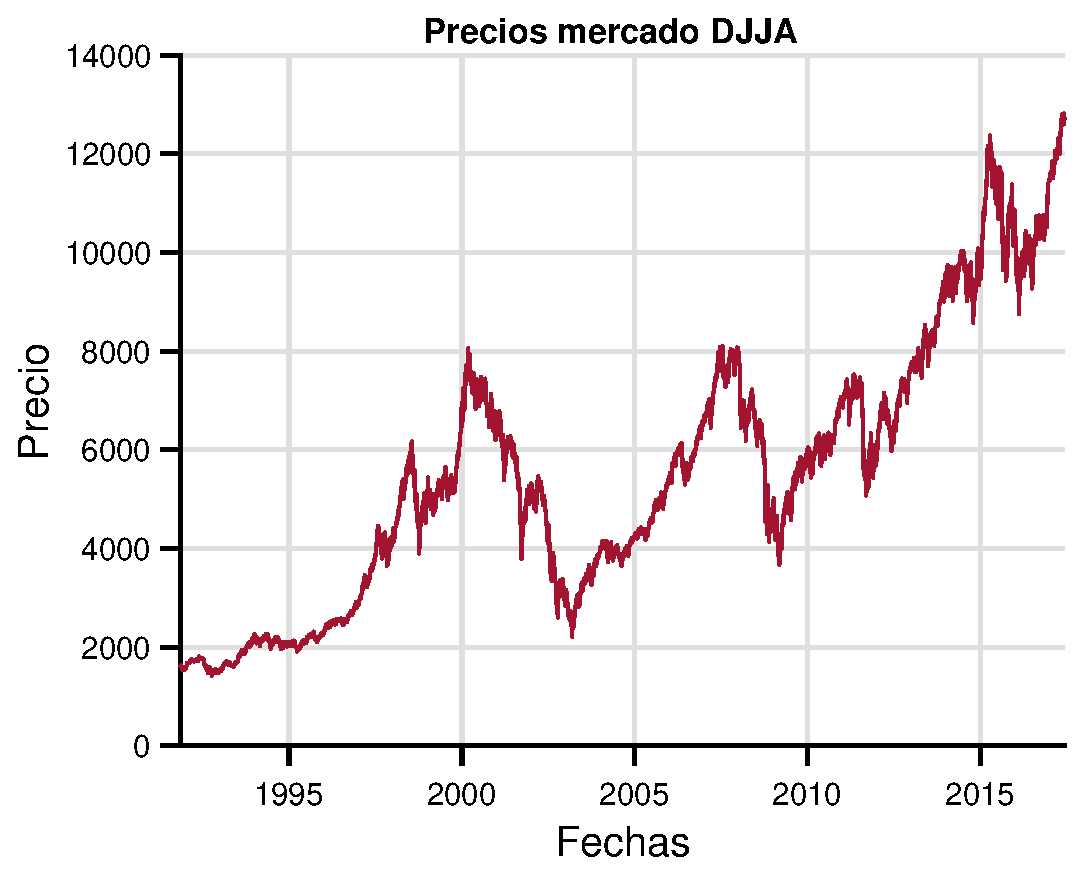
\includegraphics[width=0.7\linewidth]{figures/precioseps}
	\caption{.....}
	\label{precioseps}
\end{figure}

Se calcularon lo retornos como se explia en la section \ref{Calculo_retornos} aplicando el algoritmo \ref{diagramaentropia1}.


\begin{figure}
	\centering
	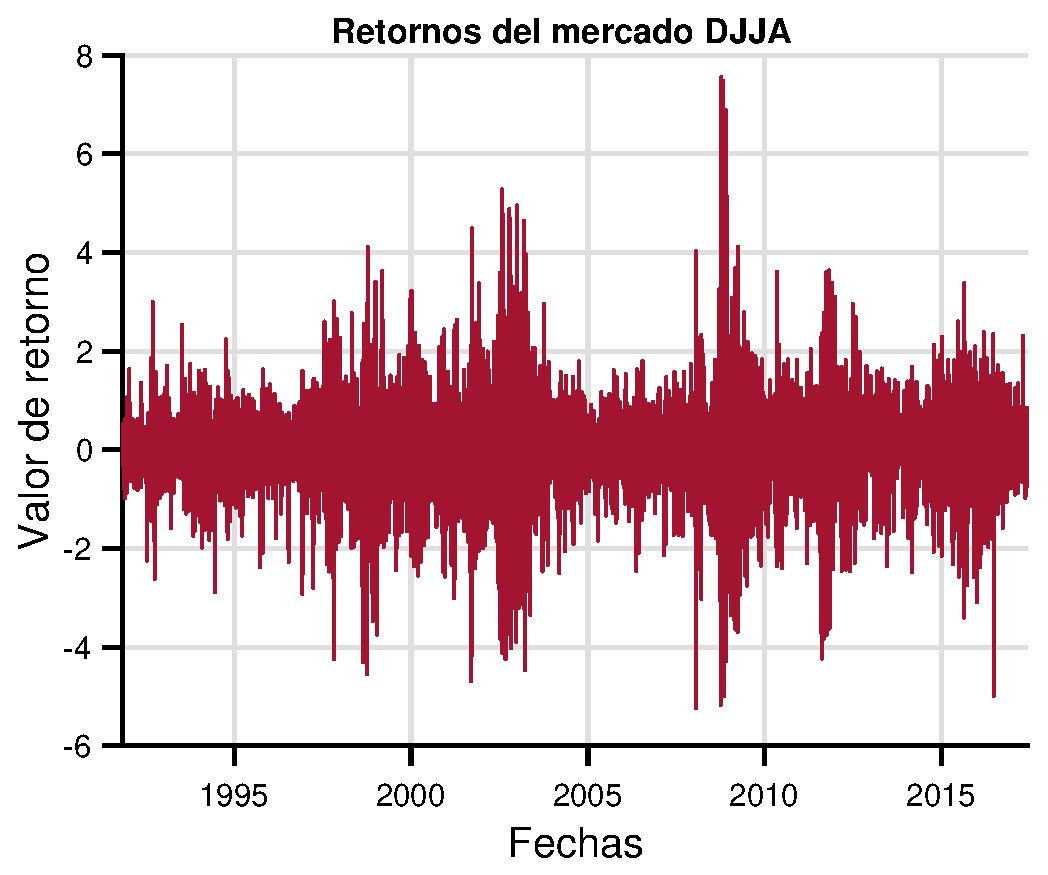
\includegraphics[width=0.7\linewidth]{figures/onlyreturnseps}
	\caption{.....}
	\label{onlyreturnseps}
\end{figure}


\begin{figure}
	\centering
	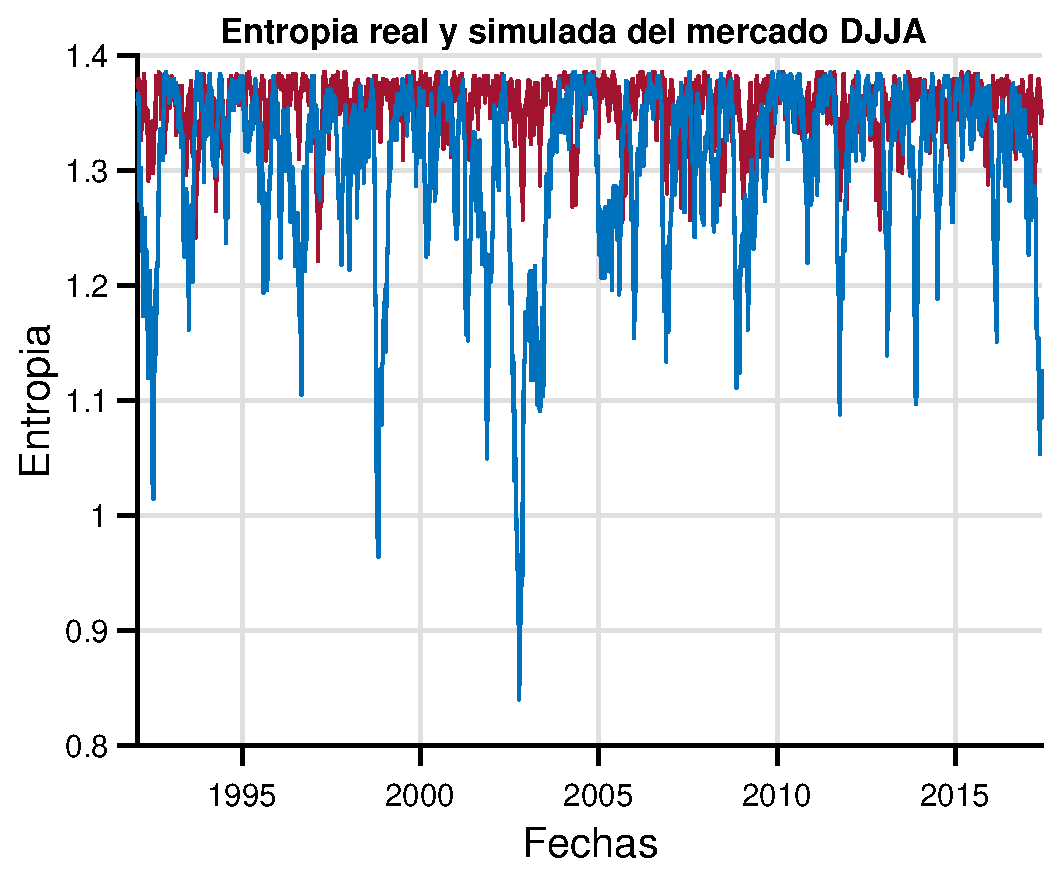
\includegraphics[width=0.7\linewidth]{figures/onlyentropyeps}
	\caption{......}
	\label{onlyentropyeps}
\end{figure}





MAV

\begin{figure}
	\centering
	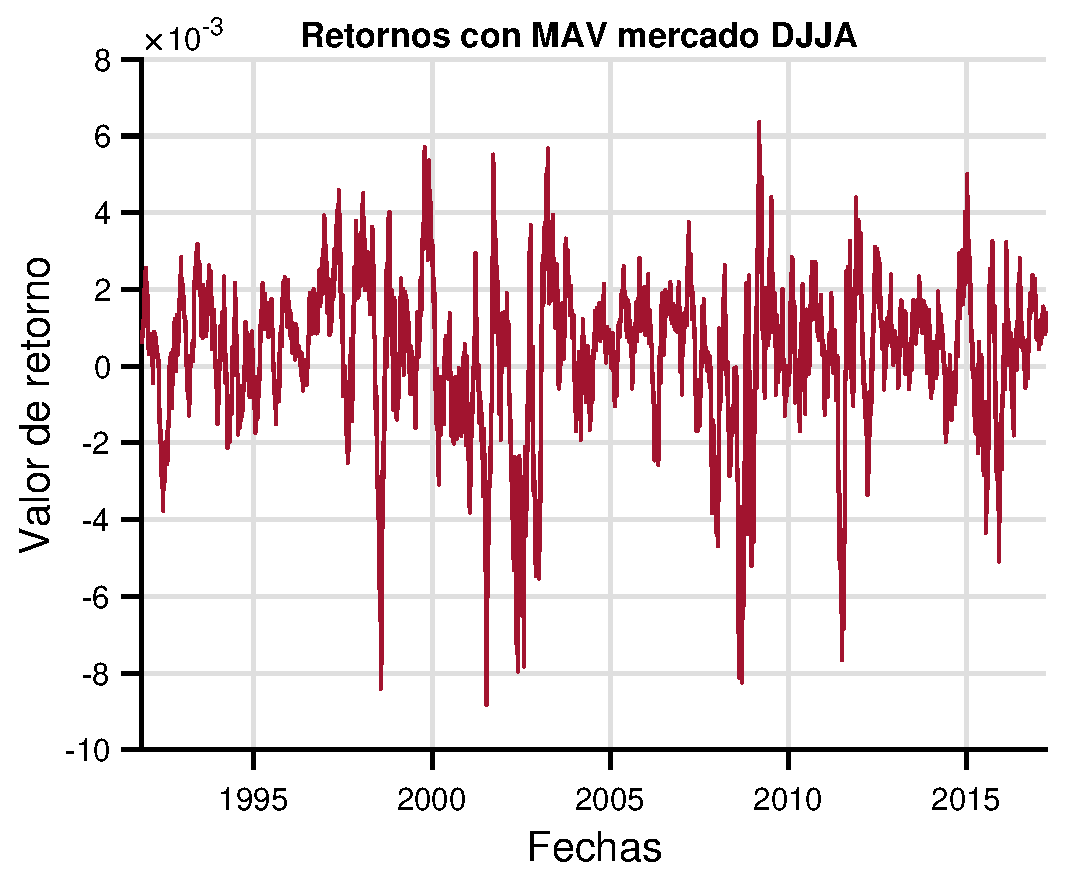
\includegraphics[width=0.7\linewidth]{figures/MAVreturnseps}
	\caption{.....}
	\label{fig:mavreturnseps}
\end{figure}



\begin{figure}
	\centering
	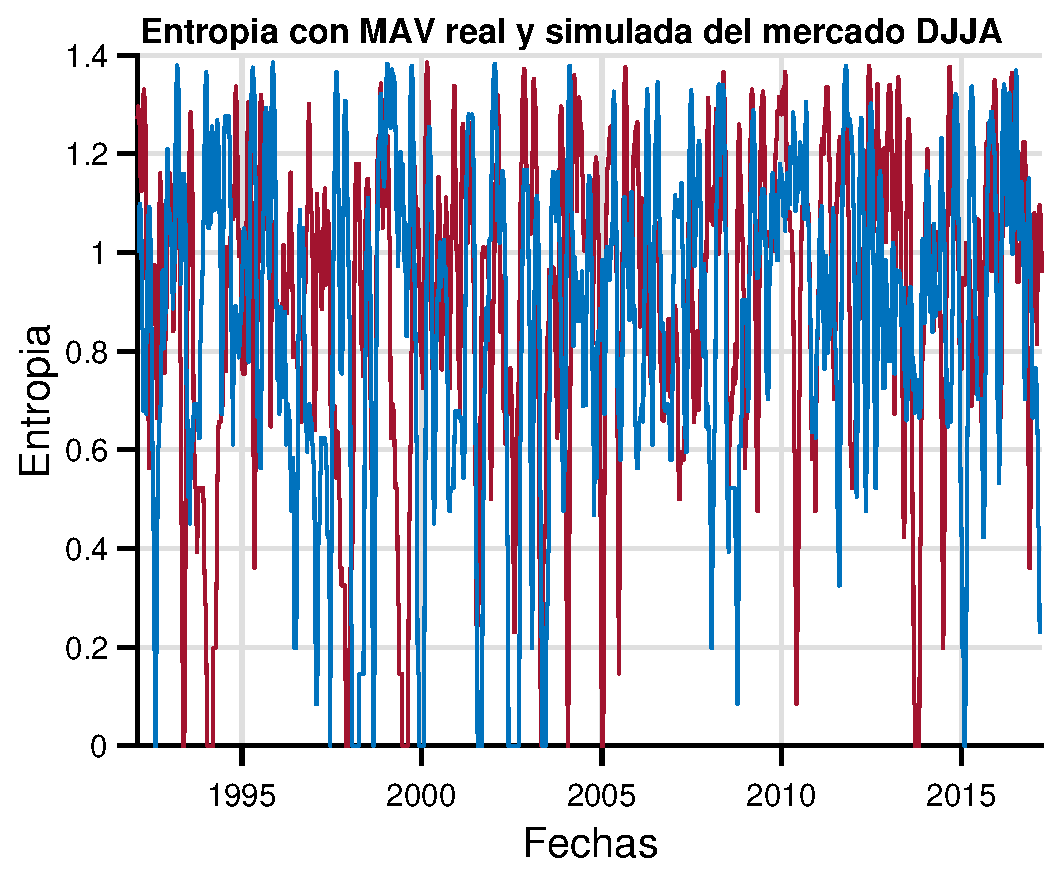
\includegraphics[width=0.7\linewidth]{figures/MAVentropy}
	\caption{}
	\label{fig:maventropy}
\end{figure}
